% !TEX root = main.tex
\chapter{Kaldi \acs{ASR} in Alex \acs{SDS}}
\label{cha:integration}

This chapter discuss the details of deploying \term{OnlineLatgenRecogniser} into Alex dialogue system.
The \term{OnlineLatgenRecogniser} is used in Alex dialogue system for Czech Public Transport Domain available on public toll-free (+420) 800 899 998 line.

First, the architecture of Alex \acf{SDS} is described.
Second, Section~\ref{sec:asrsds} presents how the wrapper \term{PyOnlineLatgenRecogniser} is integrated into~\ac{SDS} Alex.
Finally, Section~\ref{sec:eval} evaluates the decoder in Alex dialogue system on Czech \ac{PTI} domain. 

\section{Alex dialogue system architecture} 
\label{sec:arch}

The~Alex dialogue system has a~speech to speech user interface. 
The Alex dialogue system is developed in Python programming language and consists of~six major components. 
\begin{enumerate}
    \item \acf{VAD} 
    \item \acf{ASR}
    \item \acf{SLU}
    \item \acf{DM}
    \item \acf{NLG}
    \item \acf{TTS}
\end{enumerate}
The~system interacts with the user in \term{turns}. 
The schema in~Figure~\ref{fig:alex} illustrates how the user's input is processed in single turn.
The spoken input is passed to \ac{ASR} component which generates corresponding textual representation.
\ac{SLU} extracts semantic features from the text and \ac{DM} decides which response to present.
The \ac{NLG} component generates textual response from an internal representation of \ac{DM} and finally the \ac{TTS} read the text with human voice.

Each of the Alex's component runs in separate process in order parallelize the input data processing and output data generation.
The components communicates among themselves through system pipes.

\begin{figure}
    \begin{center}
    % Generated with LaTeXDraw 2.0.5
% Wed Apr 09 16:50:40 CEST 2014
% \usepackage[usenames,dvipsnames]{pstricks}
% \usepackage{epsfig}
% \usepackage{pst-grad} % For gradients
% \usepackage{pst-plot} % For axes
\scalebox{1} % Change this value to rescale the drawing.
{
\begin{pspicture}(0,-3.66)(14.64,3.66)
\definecolor{color685}{rgb}{0.11764705882352941,0.14901960784313725,0.8901960784313725}
\definecolor{color523}{rgb}{0.027450980392156862,0.25882352941176473,0.8431372549019608}
\definecolor{color34}{rgb}{0.7843137254901961,0.0784313725490196,0.23529411764705882}
\psellipse[linewidth=0.04,dimen=outer](5.55,1.51)(0.83,0.69)
\usefont{T1}{ptm}{m}{n}
\rput(5.5046873,1.425){VAD}
\psellipse[linewidth=0.04,dimen=outer](8.97,2.61)(0.83,0.69)
\usefont{T1}{ptm}{m}{n}
\rput(8.942186,2.525){ASR}
\psellipse[linewidth=0.04,dimen=outer](12.51,1.15)(0.83,0.69)
\usefont{T1}{ptm}{m}{n}
\rput(12.455312,1.065){SLU}
\psellipse[linewidth=0.04,dimen=outer](12.61,-1.51)(0.83,0.69)
\usefont{T1}{ptm}{m}{n}
\rput(12.567813,-1.595){DM}
\psellipse[linewidth=0.04,dimen=outer](5.49,-1.27)(0.83,0.69)
\usefont{T1}{ptm}{m}{n}
\rput(9.001249,-2.315){NLG}
\psellipse[linewidth=0.04,dimen=outer](9.03,0.0)(5.61,3.66)
\usefont{T1}{ptm}{m}{n}
\rput(5.4315624,-1.355){TTS}
\psellipse[linewidth=0.04,dimen=outer](9.03,-2.23)(0.83,0.69)
\usefont{T1}{ptm}{m}{n}
\rput(9.0,0.24){\Huge Dialogue System}
\psline[linewidth=0.04cm,arrowsize=0.05291667cm 2.0,arrowlength=1.4,arrowinset=0.4]{->}(9.76,2.38)(11.9,1.6)
\psline[linewidth=0.04cm,arrowsize=0.05291667cm 2.0,arrowlength=1.4,arrowinset=0.4]{->}(6.36,1.76)(8.18,2.42)
\psline[linewidth=0.04cm,arrowsize=0.05291667cm 2.0,arrowlength=1.4,arrowinset=0.4]{->}(12.54,0.46)(12.56,-0.86)
\psline[linewidth=0.04cm,arrowsize=0.05291667cm 2.0,arrowlength=1.4,arrowinset=0.4]{->}(11.84,-1.74)(9.9,-2.32)
\psline[linewidth=0.04cm,arrowsize=0.05291667cm 2.0,arrowlength=1.4,arrowinset=0.4]{->}(8.14,-2.18)(6.3,-1.52)
\pscircle[linewidth=0.04,dimen=outer](0.98404694,2.1548762){0.6451238}
\psline[linewidth=0.04cm](1.0,1.0)(0.92,-0.16)
\psline[linewidth=0.04cm](0.98193634,1.0577894)(0.0,1.84)
\psline[linewidth=0.04cm](0.98193634,1.0432783)(2.0694895,2.1461184)
\psline[linewidth=0.04cm](0.9072397,-0.23489322)(1.46,-1.72)
\psline[linewidth=0.1cm,linecolor=color523,linestyle=dashed,dash=0.16cm 0.16cm,arrowsize=0.05291667cm 2.0,arrowlength=1.4,arrowinset=0.4]{->}(2.28,1.86)(4.46,1.5)
\psline[linewidth=0.1cm,linecolor=color523,linestyle=dashed,dash=0.16cm 0.16cm,arrowsize=0.05291667cm 2.0,arrowlength=1.4,arrowinset=0.4]{<-}(2.32,-0.52)(4.36,-0.88)
\usefont{T1}{ptm}{m}{n}
\rput(3.0603125,-1.055){\Large \color{color685}Speech}
\usefont{T1}{ptm}{m}{n}
\rput(3.0803125,1.345){\Large \color{color685}Speech}
\usefont{T1}{ptm}{m}{n}
\rput(6.8231244,2.605){\color{color34}Speech}
\usefont{T1}{ptm}{m}{n}
\rput(11.20875,2.605){\color{color34}Text/Lattice}
\usefont{T1}{ptm}{m}{n}
\rput(12.445,-0.435){\color{color34}Semantic meaning}
\usefont{T1}{ptm}{m}{n}
\rput(11.265624,-2.255){\color{color34}Action}
\usefont{T1}{ptm}{m}{n}
\rput(6.899688,-2.175){\color{color34}Text}
\psline[linewidth=0.04cm](0.8872397,-0.23489322)(0.1,-1.62)
\psline[linewidth=0.04cm](0.36193633,2.0032785)(1.72,2.76)
\psdots[dotsize=0.12](1.34,2.28)
\rput{48.07518}(1.8088533,-0.49558815){\psarc[linewidth=0.04](1.46,1.78){0.12}{0.0}{180.0}}
\psline[linewidth=0.04cm](1.0368464,1.4389827)(1.0031536,1.1610173)
\end{pspicture} 
}

    \caption{Single turn in Alex dialogue system}
    \label{fig:alex} 
    \end{center}
\end{figure}

In order to prepare \ac{ASR} unit for \term{PyOnlineLatgenRecogniser} we have implemented not only the wrapper itself, but also preparation scripts and useful utilities. 
Let us introduce the Alex \ac{SDS} framework organisation, so we can better explain how our scripts are used.
The framework is separated into several logical parts:
\begin{itemize}
    \item The core library is located at \term{alex/components/}. The library is domain and language independent. All components in Figure~\ref{fig:alex} are implemented in this core library.
    \item Settings and scripts for specific domain applications are located in \term{alex/applications/}.
        For example, application for \ac{PTI} domain can be found in \term{alex/applications/PublicTransportInfoCS/} directory.
        % and started by simple scripts \term{vhub\_live\_kaldi} which starts the Alex \ac{SDS} service which provides \acl{PTI} at the 800 899 998 toll free line.
    \item The scripts which use external tools or data can be found in:
        \begin{itemize}
            \item \term{alex/corpustools/} directory which focuses on formatting and organising the collected data,
            \item and \term \term{alex/tools/} directory which stores code for modelling \ac{VAD}, \ac{ASR}, \term{SIP} client, etc.
        \end{itemize}
    \item Integration tests are stored in \term{alex/tests/}.
    \item The \term{alex/utils/} directory contains simple utilities for various purposes.
\end{itemize}

The components depicted in Figure~\ref{fig:alex} are represented as Python modules under the \term{alex/components/} directory.
The~source code of the~components is very modular, so each component may support multiple implementations.
For example the \ac{ASR} component currently supports several \ac{ASR} recognisers.
The recognisers implement a common base class \term{ASRInterface} which is presented in Listing~\ref{snippets/asr_interface.py}.
The supported speech recognisers are:
\begin{itemize}
    \item OpenJulius (\term{alex/components/asr/julius.py}) interfaces OpenJulius decoder through sockets for on-line recognition.
    \item Google (\term{alex/components/asr/google.py}) uses cloud service for batch decoding.
    \item Kaldi (\term{alex/components/asr/kaldi.py}) imports \term{PyOnlineLatgenRecogniser} class and uses its functionality for on-line decoding.
\end{itemize}

One can easily choose an \ac{ASR} recogniser in Alex configuration file.
The configuration file is also the right place to specify \ac{AM} and \ac{LM} and the speech recognition parameters if necessary.
% For example, by specifying the \ac{ASR} tool, \ac{AM} and other parameters one can choose between \ac{ASR} cloud based service, local OpenJulius or Kaldi speech recognition.

In order to prepare a specific application with \term{PyOnlineLatgenRecogniser} one need to train \ac{AM} and \ac{LM}.
One need to always train \ac{SLU} unit based on the \ac{ASR} unit outputs.
The \ac{LM} model training and consequently \ac{SLU} training is very domain specific so the scripts are deployed for each application separately.
For example, the scripts for \ac{LM} and \ac{SLU} model training for \ac{PTI} domain are located under directory \term{alex/applications/PublicTransportInfoCS/} in directories \term{lm/} and \term{slu/}.

\section[Kaldi integration into \acs{SDS} framework]{Kaldi integration into Alex's \acl{SDS} framework}
\label{sec:asrsds}

Integration of the~Kaldi real-time recognizer into Alex's framework requires implementing following features:
\begin{enumerate}
    \item The \term{kaldi.py} module which exploits functionality of \term{PyOnlineLatgenRecogniser} and implements the abstract \term{ASRInterface}.
    \item The training scripts for \acp{AM}.
        \item The scripts for building custom decoding graph \term{HCLG}.\term{HCLG} graph is a Kaldi effective representation of \ac{AM} and \ac{LM} used for decoding. 
    \item Evaluation of the \ac{ASR} recogniser in Alex, so the best speech recogniser can be selected.
\end{enumerate}

The \term{PyOnlineLatgenRecogniser} integration is described in Subsection~\ref{sub:asr_component}.
The training scripts for training \acp{AM} were described in Chapter~\ref{cha:train}.
However, note that we adjusted their directory structure and copied them into \term{alex/tools/kaldi} directory so they nicely in the Alex \ac{SDS}.
The scripts for building the \term{HCLG} decoding graph are introduced in~Subsection~\ref{sub:hclg}.
They are stored at \term{alex/applications/PublicTransportInfoCS/hclg/}.
Finally, the Section~\ref{sec:eval} evaluates the performance of \term{PyOnlineLatgenRecogniser} in Alex \ac{SDS} and briefly compares it with Google speech recognition service used through Python module \term{alex/components/asr/google.py}.

\subsection{\term{PyOnlineLatgenRecogniser} in Alex}
\label{sub:asr_component}
The \ac{ASR} component in the~Alex dialogue system runs as separate process, and the speech recognition is triggered based on \ac{VAD} decisions.

If \ac{VAD} detects start of speech in the~input audio stream, it sends the speech signal to \ac{ASR} component and the~\term{rec\_in} method is called. 
The~\term{rec\_in} method is a part of Alex abstract \term{ASRInterface} illustrated in~Listing~\ref{snippets/asr_interface.py}.
See Listing~\ref{snippets/asr_interface.py}.
In Kaldi implementation of \term{rec\_in}, the audio is decoded using beam search while the user is speaking, i.e., the method \term{rec\_in} gradually adds the new audio to \term{PyOnlineLatgenRecogniser's} buffer and immediately decodes it.\footnote{If the \ac{ASR} component is busy with decoding the audio just waits in \ac{VAD} buffer instead of in \term{PyOnlineLatgenRecogniser}'s buffer.}

If \ac{VAD} recognises end of speech, no more data are sent to \term{PyOnlineLatgenRecogniser} engine and \term{hyp\_out} method is called in order to extracted word posterior lattice.
Then, the word posterior lattice is converted to an~n-best list.\footnote{We would like to implement direct keyword spotting from \term{pyfst} lattices in Alex \ac{SLU} unit in future.}
%represented as proprietary \term{UtteranceNBlist} n-best list.

The \term{flush} method is used only if the speech recogniser wants to throw away the buffered audio input and reset the decoding.

\code{ASRInterface}{Python}{snippets/asr_interface.py}

The method \term{rec\_wav} from Alex's \term{ASRInterface} nicely illustrates how the two methods \term{rec\_in} and \term{hyp\_out} are used for decoding. 
Since the method is used only for testing purposes, it sends all input audio to the speech recogniser at once.
However, in real-time application the audio is passed to \term{PyOnlineLatgenRecogniser} in small chunks, so the decoding can run as a user speaks. 

In~the on-line Kaldi settings, latency of the~\ac{ASR} unit depends mostly on~the time spent in \term{hyp\_out} method.
In~the \term{hyp\_out} method a~word posterior lattice is extracted using the \term{PyOnlineLatgenRecogniser::GetLattice} method as described in~Subsection~\ref{sec:pyext}. 
For most cases the latency is well below 200 ms for our settings as illustrated in Figure~\ref{fig:prc}.

The~Alex dialogue system frequently handles several spoken requests immediately one after another.
It may seem that a user should wait to response of the Alex dialogue system before he speaks again and consequently new audio is buffered to recognition.
However in practice, users speak spontaneously; as first utterance is pronounced and users immediately start speaking in order to change his request.
Nevertheless, at the end of each utterance the \term{hyp\_out} method is called and the ASR hypothesis is extracted.
Since the user already speaks when the lattice is extracted, the processor time which is meant for lattice extraction can not be be used for decoding.
Consequently, the \term{rec\_in} should decode the buffered audio faster in shorter time than the~user speaks.

We noticed the problem for chains of noises detected in \ac{VAD} components as multiple short utterances.
The (\term{rec\_in} method) was extracting hypothesis while the audio input was still buffering the noisy speech and want to call \term{rec\_in}.
The~(\term{hyp\_out} method) was called so often that almost no decoding was performed.
The problem was solved by improving \ac{VAD} so the~\term{hyp\_out} method is not triggered so often.

\subsection{Building in-domain decoding graph}
\label{sub:hclg}
A decoding graph is a graph represented as an OpenFst object it stores all the \ac{LM} model information and part of information for acoustic modelling. 
The decoding graph is necessary for decoding with Kaldi decoders.
We build the \term{HCLG} graph using standard OpenFst operations which are implemented in Kaldi utilities. 

We designed our scripts so they automatically update newly built \acp{AM} and \acp{LM} and create all files necessary for decoding with \term{OnlineLatgenRecogniser} including \term{HCLG} graph.
The same files can also be used with standard Kaldi decoders or \term{PyOnlineLatgenRecogniser}.

The \term{HCLG} build script requires:
\begin{itemize}
    \item \acl{LM}
    \item \acl{AM}
    \item Acoustic phonetic decision tree
    \item Phonetic dictionary
\end{itemize}

As a results, the \term{HCLG} graph is built.
In addition, the script copies files generated by \ac{AM} training which are required for decoding with \term{PyOnlineLatgenRecogniser}.
To sum up, following files are necessary for decoding with Kaldi decoders:
\begin{itemize}
    \item Decoding graph \term{HCLG} 
    \item \acl{AM}
    \item Matrix which defines feature transformations
    \item Settings for speech parametrisation and feature transformations which match settings used for training the used \ac{AM}.
    \item \ac{WST} --- mapping between integer labels
\end{itemize}

We also developed evaluation scripts which simply compute the statistics of measures which are evaluated given \ac{AM}, \ac{LM} and parameters in~Section~\ref{sec:eval}.
Both the evaluation scripts and build \term{HCLG} script are located in the~\term{alex/applications/PublicTransportInfoCS/hclg/} directory.

\subsubsection*{Acoustic and language models for \acs{PTI} domain}
\label{sec:ptilm}
The~\term{OnlineLatgenRecogniser} is evaluated on a~corpus of audio data from the~Public Transport Information (PTI) domain.
% The phone call audio data were collected from Alex's users, so the test data simulates the real setup perfectly.
In PTI, users can interact in Czech language with a~telephone-based dialogue system to find public transport connections \cite{ptics2014url}.
The~PTI corpus consist of approximately 12,000 user utterances with a length varying between 0.4 s and 18 s with median around 3 s.
The~data were divided into training, development, and test data where the~corresponding data sizes are 9496, 1188, 1188 utterances respectively.
For evaluation, a~domain specific class-based language model with a vocabulary size of approximately 52,000  and 559,000 n-grams was estimated from the~training data.
Named entities e.g., cities or bus stops, in class-based language model are expanded before building a~decoding graph.
The~perplexity of the~resulting language model evaluated on the~development data is about 48.

Since the~PTI acoustic data amounts to less then 5 hours, the~acoustic training data was extended by additional 15 hours of telephone out-of-domain data from VYSTADIAL 2013 - Czech corpus \cite{korvas_2014}.
The~acoustic models were obtained by BMMI discriminative training with LDA and MLLT feature transformations.
% The~scripts used to train the~acoustic models are publicly available in ASDF \cite{asdf2014url} as well as in Kaldi \cite{kaldi2014url} and 
A~detailed description of the~training procedure is given in Chapter~\ref{cha:train}. 


\section{Evaluation of \term{PyOnlineLatgenRecogniser} in Alex}
\label{sec:eval}
We focus on evaluating the~speed of the \term{OnlineLatgenRecogniser} and its relationship with the accuracy of the~decoder.
% The decoding graph built from \ac{LM} and \ac{AM} described in Subsection~\ref{sec:ptilm}.
We evaluate following measures:
\begin{itemize}
    \item Real Time Factor (RTF) of decoding -- the ratio of the~recognition time to the~duration of the~audio input,
    \item Latency -- the~delay between utterance end and the~availability of the~recognition results,
    \item Word Error Rate (WER).
\end{itemize}

% DONE \todo{only non speed parameter LMW}
Accuracy and speed of the~\term{OnlineLatgenRecogniser} are controlled by the \term{max-active-states},   \term{beam}, and \term{lattice-beam} parameters \cite{povey2011kaldi}.
\term{Max-active-states} limits the~maximum number of active tokens during decoding.
\term{Beam} is used during graph search to prune ASR hypotheses at the~state level.
\term{Lattice-beam} is used when producing word level lattices after the~decoding is finished.
It is crucial to tune these parameters to obtain good results.

In general, one aims for a \ac{RTF} smaller than 1.0.
Moreover, it is useful in practice if the~RTF is even smaller because other processes running on the machine can influence the~amount of available computational resources.
Therefore, we target the~RTF with value of 0.6, which was estimated as sufficient by informal experiments.

\begin{figure*}[t]
    \begin{center}
    \includegraphics[scale=0.5]{beam_vs_rtfwer.pdf.ps}
    \includegraphics[scale=0.5]{latbeam_vs_latwer.pdf.ps}
    \caption{The~upper graph (a) shows that WER decreases with increasing \term{beam} and the~average RTF linearly grows with the~beam.
        The~growth of the~95th RTF percentile is limited at 0.6 by setting \term{max-active-states} to 2000, because the \term{max-active-states} parameters influence presumably the~worst cases with large search space.
    The~lower graph (b) shows latency growth in response to increasing \term{lattice-beam}.}
    \label{fig:wer} 
    \end{center}
\end{figure*}

We used grid search on the~test set to identify the optimal parameters values.
Figure~\ref{fig:wer} (a) shows the~impact of the~\term{beam} on the~WER and RTF measures.
In this case, we set \term{max-active-states} to 2000 in order to limit the~worst case RTF to 0.6.
Observing Figure~\ref{fig:wer} (a), we chose \term{beam} of value 13 for further experiments as this setting balances the~\ac{WER}.
Figure~\ref{fig:wer} (b) shows the~impact of the~\term{lattice-beam} on WER and latency when \term{beam} is fixed to 13.
We set \term{lattice-beam} to 5 based on Figure~\ref{fig:wer} (b) to obtain the~95th latency percentile of 200 ms, which is considered natural in a~dialogue \cite{skantze2009incremental}.
\term{Lattice-beam} does not affect WER, but larger \term{lattice-beam} improves the~oracle WER of generated lattices~\cite{povey2012generating}.
Richer lattices may improve \ac{SLU} performance.

\begin{figure*}[t]
    \begin{center}
    \includegraphics[scale=0.5]{frtf_vs_prc.pdf.ps}
    \includegraphics[scale=0.5]{lat_vs_prc.pdf.ps}
    \caption{The~percentile graphs show RTF and Latency scores for test data for \term{max-active-sates}=2000, \term{beam}=13, \term{lattice-beam}=5.
Note that 95 \% of utterances were decoded with the~latency lower that 200ms.}
    \label{fig:prc}
    \end{center}
\end{figure*}

Figure~\ref{fig:prc} shows the~percentile graphs of the~RTF and latency measures over the~test set.
The~95th percentile is the~value of a~measure such that 95\% of the~data has the~measure below that value.
One can see from Figure~\ref{fig:prc} that 95\% of test utterances is decoded with RTF under 0.6 and latency under 200 ms.
The~extreme values for 5\% of test utterances are in most cases caused by decoding long noisy utterances where uncertainty in decoding increase the search space slows down the~recogniser.
Using \term{beam} of 13, the \term{lattice-beam} of 5 and 2000 \term{max-active-states} , the~\term{OnlineLatgenRecogniser} decodes the~test utterances with a WER of about 21\%.

\begin{figure*}[t]
    \begin{center}
    \includegraphics[scale=0.5]{lat_cloud_kaldi.pdf.ps}
    \caption{Almost constant latency of on-line decoder (OnlineLatgenRecogniser) and linearly growing latency of cloud based speech recogniser (Google ASR service) for increasing utterance length.}
    \label{fig:wer} 
    \end{center}
\end{figure*}

In addition, we have also evaluated Google ASR service as we used it previously in Alex \ac{SDS}.
The~Google ASR service decoded the~test utterances from the~PTI domain with 95\% latency percentile of 1900ms and it reached WER about 48\%.
The~high latency is presumably caused by the~batch processing of audio data and network latency, and the~high WER is likely caused by a mismatch between Google's acoustic and language models and the~test data.

\subsection*{Results}
\label{sec:results}

To conclude, we implemented \ac{ASR} component based on \term{OnlineLatgenRecogniser}.
We also implemented scripts which allow easy \ac{AM} training and testing, and \ac{LM} evaluation for Kaldi speech recognition in Alex \ac{SDS}.

Based on evaluation, we selected the~best~setup\footnote{Setup: \term{beam} 12, \term{lattice-beam} 5, \term{max-active-states} 2000.} for ASR component in Alex Dialogue System Framework with  WER under 22 \%, latency less tha 200 ms and RTF under 0.6 on \ac{PTI} domain.
As a results, the~\term{OnlineLatgenRecogniser} performs significantly better than the~previous \ac{ASR} engines.
